% Name: State-space model
% Description: The block diagram of x' = Ax + Bu, y = Cx + Du, with the feedback and feedthrough paths.
% Tags: state space, control systems, linear systems

\usetikzlibrary{arrows.meta}

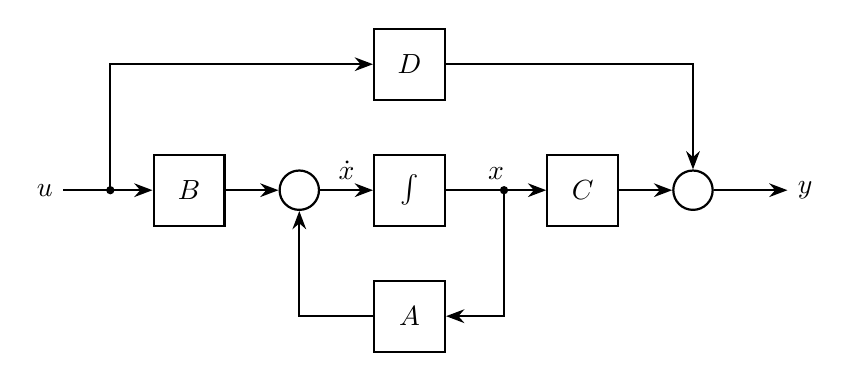
\begin{tikzpicture}[
  block/.style={draw, thick, minimum size=9mm},
  sum/.style={draw, thick, circle, inner sep=0pt, minimum size=5mm},
  arrow/.style={-{Stealth}, thick},
]
  \node[block] (B) at (1.6,0) {$B$};
  \node[sum] (s1) at (3,0) {};
  \node[block] (int) at (4.4,0) {$\int$};
  \node[block] (C) at (6.6,0) {$C$};
  \node[sum] (s2) at (8,0) {};
  \node[block] (A) at (4.4,-1.6) {$A$};
  \node[block] (D) at (4.4,1.6) {$D$};

  \draw[thick] (0,0) node[left] {$u$} -- (0.6,0);
  \draw[arrow] (0.6,0) -- (B);
  \draw[arrow] (B) -- (s1);
  \draw[arrow] (s1) -- node[above] {$\dot{x}$} (int);
  \draw[arrow] (int) -- node[above] {$x$} (C);
  \draw[arrow] (C) -- (s2);
  \draw[arrow] (s2) -- (9.2,0) node[right] {$y$};
  \draw[arrow] (5.6,0) |- (A);
  \draw[arrow] (A) -| (s1);
  \draw[arrow] (0.6,0) |- (D);
  \draw[arrow] (D) -| (s2);
  \fill (0.6,0) circle (1.5pt) (5.6,0) circle (1.5pt);
\end{tikzpicture}
